% Chapter Template

\chapter{Analysis and Discussion} % Main chapter title

\label{AnalysisAndDiscussion}

\lhead{Chapter \ref{AnalysisAndDiscussion}. \emph{Analysis and Discussion}}

%----------------------------------------------------------------------------------------
%	Design Research
%----------------------------------------------------------------------------------------
\section{Comparing the algorithms}
\label{ComparingAlgorithms}
To compare the two algorithms we generated a list of english nouns
which we sent through the lexitags server to get synsets that corresponded to the meanings of each word.
Both these lists were preprocessed to remove duplicates and to format them as javascript objects
\footnote{\url{https://github.com/EivindEE/Madame/tree/master/testing}}.
The final list of synsets contained 4350 unique synsets.
We wrote a short script that we used to run the synsets through the best fit algorithms,
and write a report of the results.
For the schema.org version of the test we wrote the average depth of the mapped type,
as well as the total number of times the two algorithms had the same and different mappings.
The debth was calculated as the distance from the root node in the tree,
i.e. schema:Thing it self had a depth of 0,
schema:Person which inherits directly from schema:Thing has a depth of 1 and so on.
For the SUMO version the depth of each type was unavailable,
so we only have numbers showing the agreement between the algorithms.
The full results from the tests can be found at the URL \url{https://github.com/EivindEE/Master-thesis/tree/master/AlgComparison}.

As one can read from the numbers it table \ref{table:AlgorithmResults} the results from the SUMO test
display no difference between the two algorithms when mapping from WordNet to SUMO.
The two algorithms return identical mappings in 100\% of the test cases.
This indicates that there must have beena mapping either directly from the synset,
or from the direct hypernym of the synset for each of the 4350 synsets in our test.
This makes it hard to say anything relevant about the algoritms from these results.

The schema.org results are more interesting.
The two algorithms still perform fairly equally.
Reading from table \ref{table:AlgorithmResults} we can see that the algorithms are equal in 75\% of the cases,
but we can examine the 25\% that are different and see which perform better in those cases.
We can also see that the algorithms were unable to find a mapping in 13.7\% of the cases.
These cases can't tell us much about which algorithm we should prefere,
but could be a good starting point for finding parts of the WordNet to schema.org mapping which could be enhanced.

Our predictions beforhand was that the hypernymes first approach would have fewer incorrect mappings,
but would give results at a more shallow depth.
The last prediction was the easiest to test, as we know the schema.org hierarchy and can calculate the depth of each type.
For each mapping we registered the depth of the type in the schema.org hierarchy.
These depths were averaged over the total number of mappings made.

As seen in table \ref{table:AlgorithmComparison} both algorithms map fairly high in the hierachy.
The hypernymes first approach maps to a type at level 0.69 on average when considering all the synsets,
or to a type at level 0.72 when ignoring the cases where the two algorithms gave the same result.
As predicted the hypernym then siblings approach does a little better, though not much,
mapping to types at level 0.8, or 1.2 when excluding identical mappings.
Looking at the data it is obvious that the hyponymes first approach much more frequently leads to mappings to Thing and Intangible.
The hypernym first algorithm maps to schema:Thing 449, and schema:Intagible 481 times,
while hypernymes then siblings maps to schema:Thing 334 and schema:Intangible 81 times.
Neither schema:Thing nor schema:Intangible are very interesting mappings in the ontology.
As described in \ref{schemadotorg}, Thing is the most general category, meaning that every concept belongs to this category.
Intangible is described\footnote{\url{http://schema.org/Intangible}} as "a utility class that serves as the umbrella for a number of 'intangible' things",
and does not have any special properties in the ontology.
Even if these mappings are quite uninteresting it is not always obvious that there are types in schema.org which are better fits for the synsets.

To judge the correctness of the algorithms,
we went through the results from when the two algorithms gave different mappings and checked the mappings manually.
The process consisted of looking up each synset that was mapped,
and the types it had been mapped to and check if the two corresponded.
The results were divided into three categories.
If it was clear that the synset and type corresponded, they were marked as correct.
If it was clear that they didn't correspond they were marked as incorrect.
There were also some cases where it was unclear whether or not a mapping were correct.

We decided it was necessary to include a category for unclear mappings to highlight the fact that some of the categories
are fuzzy and require some more documentation,
or that they might entail things than seem unnatural.
One of the instances were it was unclear if a mapping should be judged to be correct was for the mapping of dairy\#n\#1,
"a farm where dairy products are produced", which mapps to schema:FoodEstablishment.
Schema:FoodEstablishment is described as "[a] food-related business", which a dairy most certainly is.
The sub typing of schema:FoodEstablishment however seems to indicate otherwise.
The sub types of schema:FoodEstablishment are:
\begin{itemize}
	\item Bakery
	\item BarOrPub
	\item Brewery
	\item CafeOrCoffeeShop
	\item FastFoodRestaurant
	\item IceCreamShop
	\item Restaurant
	\item Winery
\end{itemize}
This seems to indicate an establishment where private customers come to purchase goods,
making a more industrial venue seem out of place.
Another schema.org term that provided some difficulty was schema:Place,
which has the description "[e]ntities that have a somewhat fixed, physical extension".
Again the sub types seem to indicate that it should be used for geographical sections.
From the description of the type it is unclear if it can be used to describe things like borders and edges of things.

Since the manual inspection of the mappings was a time consuming process we decided to only inspect 250 mappings,
and see if the results of checking these would be sufficient to say anything about the algorithms.
We excluded mappings the schema:Thing and schema:Intangible, as one could normally argue reasonably for these.

We had predicted a higher error rate in the hypernym then sibling algorithm,
but the difference in the error rate between the algorithms was much larger than we had anticipated.
Again pointing to table \ref{table:AlgorithmComparison} we can see that the hypernyms first algorithm
made correct mappings in 94\% of the test cases,
while giving incorrect mappings in 2.0\% test cases and questionable mappings in 4\% of the cases.
The hypernym then sibling algorithm on the other hand gave a correct mapping in only 26.8\% of the cases checked.
It gave incorrect mappings in 62.4\% and unclear mappings in 20.8\% of the cases.
The fact that it gave correct mappings at a rate of close to 25\% of the instances where the results were different was very surprising.
This high degree of incorrect mappings indicates that using sibling synsets as the basis for mapping in unfruitful.
We will however examine the incorrect mappings of both algorithms to try to uncover the causes,
and if they are caused by weaknesses in the algorithms, or in WordNet or the mapping from WordNet to schema.org.


The fact that the hypernyms first algorithm gave incorrect mappings at all are a bit alarming.
As described in section \ref{Hypernymy} about hyper- and hyponymy, hypernymy should be a transitive "type of" relation.
Each hypernym should then be a more general type of the synset provided and not break the semantics of the synset.
The mappings from WordNet to schema.org indicate that the semantic content of the synset are equal to the
semantic content of the schema.org type mapped to.
Since both hypernymy and mappings should preserve the semantics of the synsets, the mappings should be correct.
The fact that the hypernyms first algorithm gives incorrect mappings indicate that either the integrity of the hypernym relation is broken,
or that the mappings are incorrect.


%%%%% There were six cases
%% Rewrite and update
All the cases where the hypernyms first approach was deemed to have incorrect mappings were instances where the synset
mapped to schema:Quantity via their hypernym measure\#n\#2 \{measure, quantity, amount\}.

The hypernym chain linking birth\#n\#1, death\#n\#5, death\#n\#4 and end\#n\#2 to measure\#n\#2 ended with:
\begin{verbatim}
	beginning#n#2 / end#n#2
	point#n#6
	measure#n#2
\end{verbatim}

and birthday\#n\#2 had the chain:
\begin{verbatim}
	date#n#1
	day#n#1
	time_unit#n#1
	measure#n#2
\end{verbatim}


In schema.org the type Quantity is described as "[q]uantities such as distance, time, mass, weight".
The synset measure\#n\#2 is described as "how much there is or how many there are of something that you can quantify".
The mapping between these appear reasonable and do not seem to be the cause of error.

What makes the mappings seem unreasonable is that the synset one starts with in some way or another points towards
something that happens at a single instance in time.
A birth or death is just a single instance, not a quantity of things.
The problem in both these chains seem to be that one goes from something that happened at a single instance in time,
to a collection of things.
The cause of the error then seems to be an inconsistency within the hypernym relation in WordNet.
We will contact the maintainers and ask if they agree.

We also analysed the results where the hypernym then siblings algorithm mapped incorrectly.
The distribution of incorrect mappings can be seen in figure \ref{fig:incorrect}(page \pageref{fig:incorrect}).

\begin{figure}[ht]
	\centering
    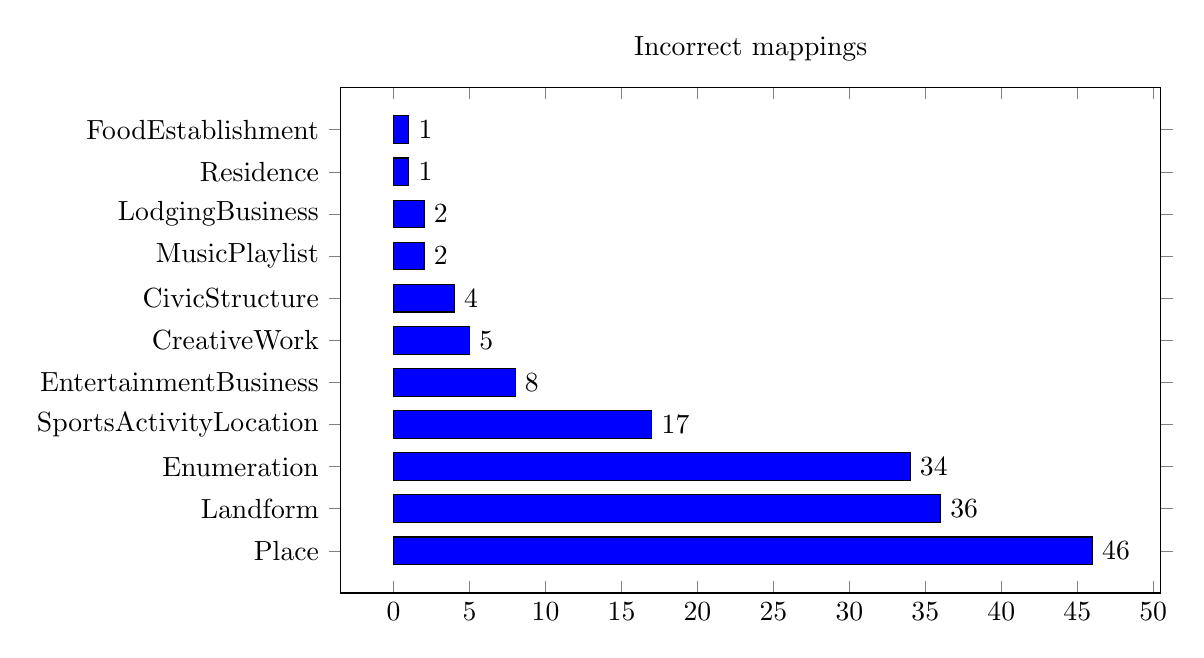
\begin{tikzpicture}
        \begin{axis}[
	        title={Incorrect mappings},
            xbar,
            width=12cm, height=8cm,
            symbolic y coords={Place,Landform,Enumeration,SportsActivityLocation,EntertainmentBusiness,CreativeWork,CivicStructure,MusicPlaylist,LodgingBusiness,Residence,FoodEstablishment},
            ytick=data,
            nodes near coords, nodes near coords align={horizontal},
          ]
            \addplot[fill=blue] coordinates {
               (46,Place)
               (36,Landform)
               (34,Enumeration)
               (17,SportsActivityLocation)
               (8,EntertainmentBusiness)
               (5,CreativeWork)
               (4,CivicStructure)
               (2,MusicPlaylist)
               (2,LodgingBusiness)
               (1,Residence)
               (1,FoodEstablishment)
            };
        \end{axis}
    \end{tikzpicture}
	\caption{Distribution of incorrect mappings in hypernym then siblings algorithm}
	\label{fig:incorrect}
\end{figure}

We picked the two most common incorrect mappings as objects of further study.
We went through all the cases of incorrect mapping to schema:Place.
This examination showed that in 45 of the 46 cases the mapping to schema:Place came as a result of
the synset being a hyponym of whole\#n\#2, which has the sibling geological\_formation\#n\#1 which again has a mapping to
schema:Landform, a sub type of schema:Place.
The last instance is the mapping from attention\#n\#3 which has the sibling tourist\_attraction\#n\#1 mapping to
schema:TouristAttraction.

For the mappings to schema:Landform all of the incorrect mappings came as a result of the synsets being hyponyms of
part\#n\#3, which has the sibling synset body\_of\_water\#n\#1 mapping to schema:BodyOfWater which is a sub type of
schema:Landscape.
Common for all these mappings is that the hypernyms are reasonable.
There is no reason to believe that these are cases where the hypernym chain breaks the semantics of the synset.
The mappings from WordNet to schema.org also seem to be sound.
This means that the source of the change in semantics must be looking at the siblings of the synset or its hypernyms.
There were instances of siblings both of the original synset and of the hypernyms,
so it does not appear that closeness to the synset needs to have any influence on whether or not the sibling gives
an accurate mapping for the synset.

\begin{table}[h] %%%% Should I change the results so that the no results found are ignored?
	\centering
	\begin{tabular}{lll}
										& Schema.org	& SUMO			\\
		Total number of synsets tested 	& 4350			& 4350			\\
		Number of identical mappings 	& 3262 (75\%)	& 4350 (100\%)	\\
		Number  of different mappings	& 1088 (25\%)	& 0	(0\%)		\\
		No result found					& 598  (13.7\%)	& 0	(0\%)
	\end{tabular}
	\caption{The testing results}
	\label{table:AlgorithmResults}
\end{table}

\begin{table}[h]
	\centering
	\begin{tabular}{lll}
											& Hypernyms First 	& Hypernym then siblings	\\
		\emph{For all mappings}				&					&							\\
		Avg. depth total					& 0.688506 			& 0.804138					\\
		\emph{For different mappings}		&					&							\\
		Avg. depth different				& 0.721507			& 1.183823					\\
		Mappings to "Thing"					& 449				& 334						\\
		Mappings to "Intangible"			& 481				& 81						\\
		\emph{For the 250 examined mappings}&					&							\\
		Correct mappings					& 235				& 67						\\
		Correct mapping	rate				& 94\%				& 26.8\%					\\
		Unclear								& 10				& 27						\\
		Unclear	rate						& 4\%				& 20.8\%					\\
		Errors								& 5 				& 156 						\\
		Error rate							& 2\%				& 62.4\%					\\
	\end{tabular}
	\caption{Comparison of the mapping algorithms}
	\label{table:AlgorithmComparison}
\end{table}

\subsection{Choosing an algorithm}
From the previous discussion and from the results of the testing it seemed clear that the hypernyms first algorithm is
the dominant strategy for mapping synsets to schema.org, and that there is no difference between the two when mapping to SUMO.
The algorithms performed very differently when mapping to the different ontologies.

It might be that an increase in the number of mappings would change the results.
One could then try to refine the hypernym then siblings algorithm to analyse the mappings of its siblings,
and try to find some more sophisticated way of choosing which mapping to select.

It would also be interesting to try mapping to a more general ontology than schema.org.
As mentioned in section \ref{schemadotorg} schema.org is a small ontology with only 577 types,
and with a bias towards comercial interests.
It might be that an ontology that was larger,
and which had a more balanced approach to the world would result in better results for the algorithm.

As it stands it is clear that the hypernyms first algorithm out performed the hypernym then siblings algorithm,
and is the one that will be used in the artefact.
The fact that its mappings were incorrect or questionable in 6\% of the instances analyzed is unfortunate.
We have however analysed the reason for these errors and should have enough information to improve the results further.
%Noun list from http://www.desiquintans.com/articles.php?page=nounlist

%https://github.com/EivindEE/Master-thesis/blob/master/AlgComparison/AlgComparisonResultsBig
%https://github.com/EivindEE/Master-thesis/blob/master/AlgComparison/compare-different

\section{Testing against existing markup}
One of our success criteria was that it should be posible to markup HTML as well or better than what is on the web now.
To find webpages that uses schema.org as an ontology for adding metadata we used a list found on github of
this type of sites\footnote{\url{https://github.com/LawrenceWoodman/mida/wiki/Sites-Using-Microdata}}.
The process we used consisted of opening the sites and seeing what metadata the site we tested had,
and then open the site using \theartefact and try to add the same metadata.
We would then analyse the results by using Googles structured data testing tool
\footnote{\url{http://www.google.com/webmasters/tools/richsnippets}},
and W3s RDFa 1.1 distiller and parser\footnote{\url{http://www.w3.org/2012/pyRdfa/}}
to confirm that the metadata was added and was correct.
The webpages were also checked without being enhanced with the tool to see if they were structured correctly.

The pages we marked up where:
\begin{itemize}
	\item A restaurant review from the Telegraph\footnote{\url{https://github.com/EivindEE/Master-thesis/blob/master/WildTesting/Bunga\%20Bunga\%2C\%20London\%2C\%20restaurant\%20review\%20-\%20Telegraph.html}}
	\item A tour operators customer feedback page\footnote{\url{https://github.com/EivindEE/Master-thesis/blob/master/WildTesting/Customer\%20Feedback\%20\%7C\%20About\%20Us\%20\%7C\%20The\%20Holiday\%20Place.html}}
	\item A tourist agency home page \footnote{\url{https://github.com/EivindEE/Master-thesis/blob/master/WildTesting/Luxury\%20Travel\%20Africa\%20\%7C\%20Best\%20South\%20Africa\%20Tour\%20Operator\%20\%7C\%20Luxury\%20Safari.html}}
	\item The home page of a marketing company \footnote{\url{https://github.com/EivindEE/Master-thesis/blob/master/WildTesting/Internet\%20Marketing\%20Experts\%20helps\%20you\%20get\%20MORE\%20business\%20from\%20the\%20Internet\%20\%7C\%20Ebizindia.html}}
	\item A movie review sites review of a film \footnote{\url{https://github.com/EivindEE/Master-thesis/blob/master/WildTesting/Punching\%20The\%20Clown\%20Movie\%20Review\%20-\%20Media\%20Decay.html}}
\end{itemize}

Most of the metadata on the webpages that were marked up were metadata about larger sections of the page.
The most prevalent type used on the pages we marked up was schema:Review.
The artefact we developed is targeted towards disambiguating single words as described in section \ref{Interaction}.
This mismatch means that the preferred interaction of highlighting text and selecting one of the posible
disambiguations of the selection is unavailable.
Instead we had to rely on the fallback interaction which uses the original highlighting for finding the range of
the selection to tag, and user input in the form of writing what the topic of the selection is.
This process is functional, but is more cumbersome than the originally intended interaction.


We found the results to be satisfactory, and were able to recreate all the metadata that was present on the webpages
we decided to test against, with the exception of aggregate type mappings which we will discuss bellow.

The originals of the webpages that were used to test the tool were considered the gold standard which we used to
evaluate the result of the mapping.
The exception we had to this was when the webpages used invalid types or properties in their metadata.
In the pages we checked we found one instance of invalid metadata.
On the page with the movie review we found that the author of the HTML had added an invalid property to a movie.
The webpage used the property name "publishdate" while the correct name of the property is "datePublished".
An advantage of using a tool like \theartefact is that one can be sure not to use incorrect properties such as this,
since the tool provides a list which only contain valid properties for the type one has selected.


We found that there are some schema.org types that we are not able to reach with the current systems.
In particular we have found out the the system does not have a way to reach aggregated types.
At the time of writing the aggregate types in schema.org are schema:AggregateRating and schema:AggregateOffer.
The type schema:AggregateRating is meant to represent the average rating that a rated object has received
while schema:AggregateOffer represents a collection of offers for a given product.
The difficulty posed by both these types is that what separates them from their super types schema:Rating and schema:Offer
is that they represent the plurality of the super type.
The system uses WordNet to represent and disambiguate words, and as its basis for mapping natural language to ontologies.
WordNet is a dictionary type system, which does not separate between the different grammatical numbers of a given word,
as they all represent the same concept.
For the system this is a problem, since it means that the language we use as an intermediary between natural language
and the ontologies does not capture all of the complexity of the ontologies we wish to map to.


Another issue we came across when analyzing the resulting markup with the the structured data tool was that we got
error messages saying that some of the elements that had been marked up were missing required properties.
This is problematic for two reasons.
On is that it greatly increases the complexity of the system,
as it increases the minimum amount of work a user has to do to get valid metadata,
and requires the system to give the user additional cues regarding the validity of the metadata.
Cues that the user needs to be taught to successfully use the system.
The other problem is that the fact that these properties are required is undocumented.
When analyzing a schema:Product without a name value the error message reads:
\begin{verbatim}
	Warning: Missing required field "name (fn)".
	Warning: Incomplete rdfa with schema.org.
\end{verbatim}
The documentation on the schema.org homepage does not give any indication that schema types have required properties.
When looking closer at the unmodified web pages it was revealed that when using the microdata format these types
were ignored without warning.
The fact that the validator requires the properties does not in it self mean that the markup is incorrect,
or that the syntax is wrong.
The validator seems geared towards the generation of rich snippets,
and it might be that the warning is intended to warn that the amount of metadata is insufficient to generate rich snippets.
%% Problem, missing required properties, not documented as required by schema.org

%% Punching The Clown Movie Review - incorrect property

\section{Suitability of WordNet for mapping natural language}
